\documentclass[11pt,nofootinbib]{revtex4}
\usepackage[utf8]{inputenc}
\usepackage{natbib}
\usepackage{float}
\usepackage{graphicx}
\linespread{1}

\usepackage{listings}
\lstset{frame=tb,
  language=sh,
  aboveskip=3mm,
  belowskip=3mm,
  showstringspaces=false,
  columns=flexible,
  basicstyle={\small\ttfamily},
  numbers=none,
  numberstyle=\tiny\color{gray},
  keywordstyle=\color{blue},
  commentstyle=\color{green},
  stringstyle=\color{mauve},
  breaklines=true,
  breakatwhitespace=true,
  tabsize=3,
  mathescape = true,
}

\usepackage{hyperref}
\hypersetup{
    colorlinks=true,
    linkcolor=blue,
    filecolor=magenta,      
    urlcolor=cyan,
}

\newcommand{\dollar}{\mbox{\textdollar}}

\begin{document}

\title{Using SUMO to Validate Mixed Autonomy Road Capacity Models}
\author{David Rower}
\affiliation{Department of Physics, University of California Santa Barbara, Santa Barbara CA 93106}

\maketitle

\section{Motivation and Scope}
This report was created with two goals: to detail some simple simulation studies validating two mixed autonomy road capacity models presented in Lazar et al. \cite{Lazar1} and to provide some basic knowledge of the microscopic traffic simulator SUMO used to validate the models. We present a brief overview of the capacity models and SUMO configuration, and a terse discussion of some simulation artifacts. We also offer a guide to replicate the specific build of SUMO used in these studies in the appendix.

\section{Road Capacity Models}
\subsection{Capacity Model 1}
In this model, an autonomous vehicle is indiscriminate in reducing its headway when following other vehicles. Let $m$ be the capacity of the road when fully utilized by regular vehicles, and $M$ be the capacity of the road when fully utilized by autonomous vehicles. Let $\alpha$ be the average proportion of smart vehicles on the road. The capacity of the road under autonomy level $\alpha$ is approximated by 
\begin{equation}
    C(\alpha) = \frac{1}{\alpha M^{-1} + (1-\alpha)m^{-1}}. 
\end{equation}

Note that, for a single lane road of length $d$, where regular vehicles assume headway $h_{r}$ and autonomous vehicles assume headway $h_{s}$, we have $M = d/h_{s}$ and $m = d/h_{r}$. Let the length of every vehicle be $l$. We can then express the capacity as 
\begin{equation}
    C(\alpha) = \frac{d}{\alpha h_s + (1-\alpha)h_r + l}. 
\end{equation}

The physical significance of $h_r$ and $h_s$ can be appreciated below in Fig. \ref{headways_1}. 
\begin{figure}[h]
\centering
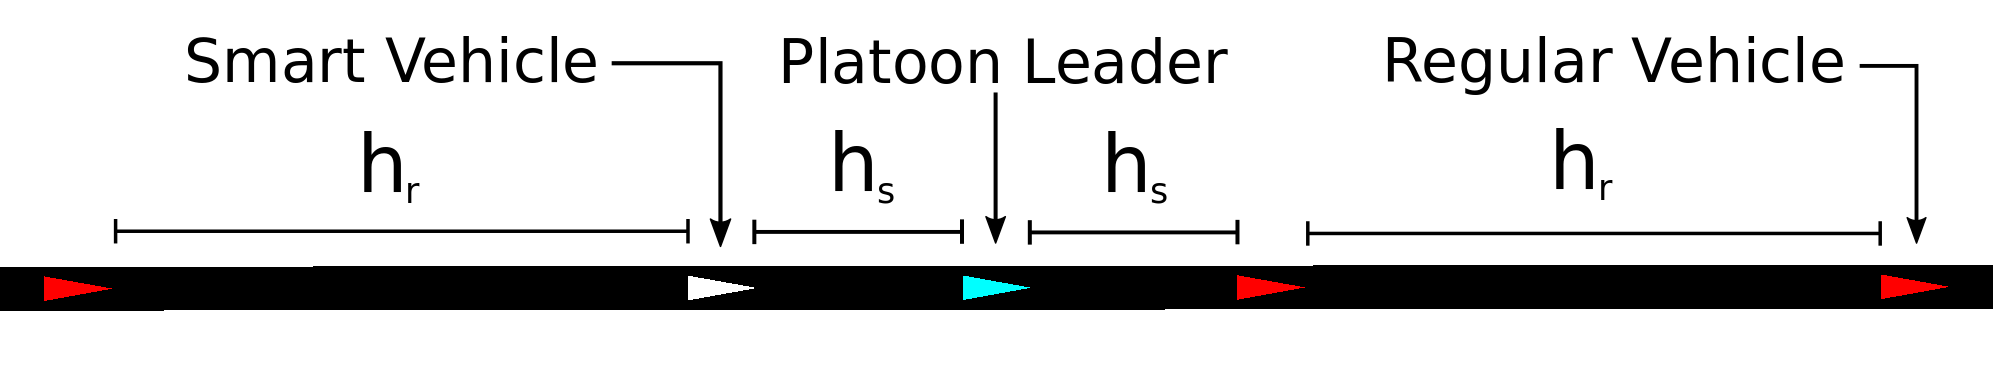
\includegraphics[width = 100mm]{images/headways_model1.png}
\caption{A representation of car interactions in SUMO according to capacity model 1. In this model, an autonomous vehicle will always follow with a distance $h_s$ to the car in front of it. A regular vehicle will follow with headway $h_r$.}
\label{headways_1}
\end{figure}

\subsection{Capacity Model 2}
In this model, an autonomous vehicle adjusts its headway according to the technology of the car it is following; it only reduces its headway when following another autonomous vehicle. Using the same notation as above, we have
\begin{equation}
    C(\alpha) = \frac{1}{\alpha^2 M^{-1} + (1-\alpha^2)m^{-1}} = \frac{d}{\alpha^2 h_r + (1-\alpha^2)h_s + l}. 
\end{equation}

The physical significance of $h_r$ and $h_s$ can be appreciated in Fig. \ref{headways_2} below. 
\begin{figure}[h]
\centering
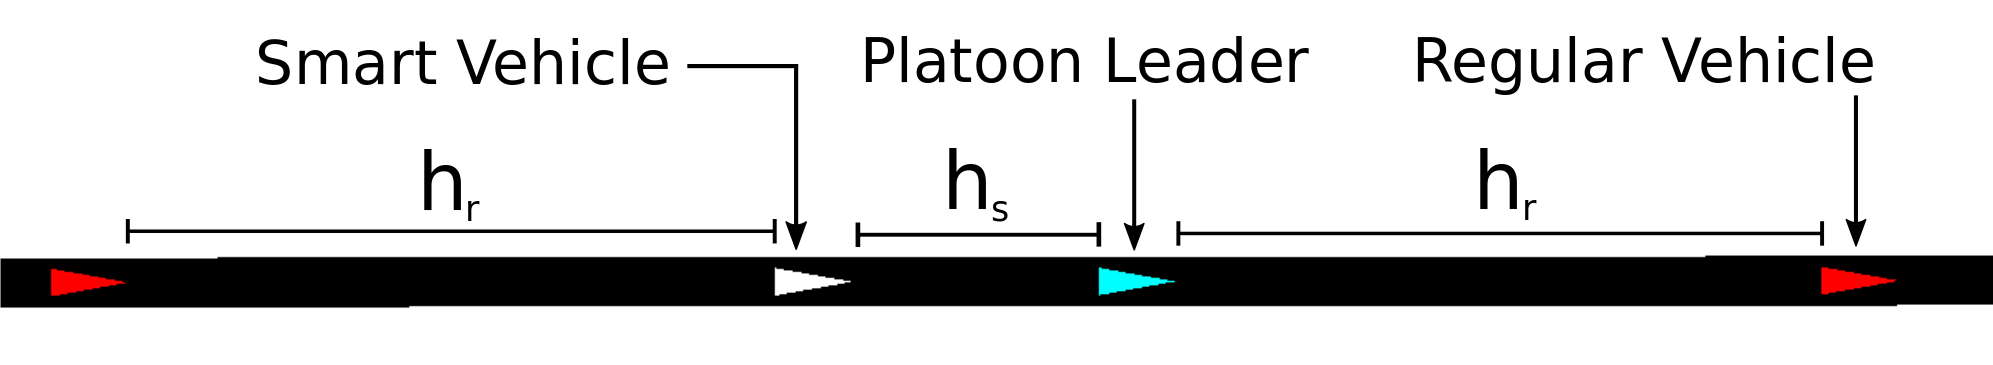
\includegraphics[width = 100mm]{images/headways_model2.png}
\caption{A representation of car interactions in SUMO according to capacity model 2. In this model, an autonomous vehicle will only follow with a distance $h_s$ to the car in front of it if that car is also autonomous. A regular vehicle will always be followed with distance $h_r$.}
\label{headways_2}
\end{figure}


\section{Validation of Models In SUMO}

\subsection{SUMO Configuration}
The most basic road network was used to validate the capacity models - a single-lane road in a straight line. Below, we outline the basic configuration files needed to define this scenario. 

\begin{enumerate}
    \item \verb|/single_road/network/single.net.xml|
    \begin{itemize}
        \item This file defines the road graph, including the locations of vertices in a plane, the edges between vertices, and the speed limit along those edges. 
    \end{itemize}
    \item \verb|/single_road/network/single.rou.xml|
    \begin{itemize}
        \item Types of vehicles are defined here according to a car following model, color, acceleration parameters, impatience, length of vehicle, maximum speed, minimum gap from vehicle immediately in front, and headway. 
        \item Instances of these vehicles on the road are also defined here. This can be done in multiple ways, but for this study it was useful to define a "flow," where a proportion of different vehicle types is specified and the traffic is generated from this distribution. 
    \end{itemize}
    \item \verb|/single_road/network/single.det.xml|
    \begin{itemize}
        \item This file defines sensors on the road, including the locations of the sensors on specific edges of the road graph, the frequency of detection, and the output files. Note that the output files weren't necessary, as an interface from Python was available to directly talk to these sensors. 
    \end{itemize}
\end{enumerate}

An example of a sensor in the graphical rendering of SUMO is presented in Fig. \ref{sensor}. 
\begin{figure}[H]
\centering
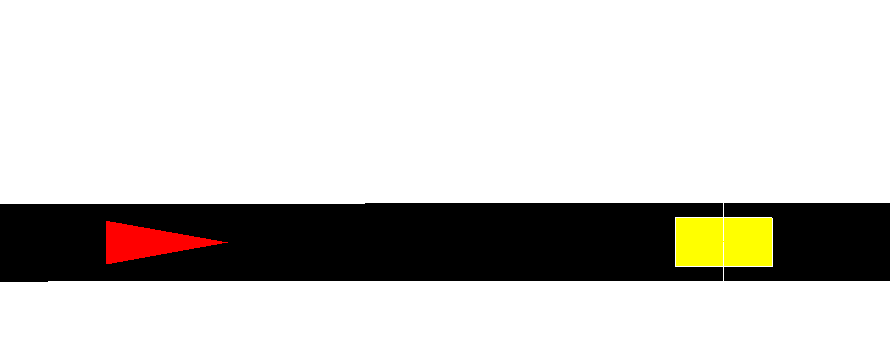
\includegraphics[width = 50mm]{images/sensors.png}
\caption{A sensor as displayed in the GUI of SUMO. The yellow box is the sensor, which can be listened to directly through a Python script. The red triangle represents a car.}
\label{sensor}
\end{figure}

\subsection{Overview of TraCI}
In order to gather data quickly and effectively from SUMO, TraCI, a "Traffic Control Interface," was released. TraCI allows you to directly observe and manipulate instances of SUMO via several supported programming languages, including Python. This was used to automate the running of several instances of SUMO, and to collect data from each of those instances. 

\subsection{Our Scenario}
A single-lane road in a straight line was defined, and two sensors were defined along the road. One sensor was placed roughly 1/5 of the way down the road, the other was placed near the end of the road (but not at the end, as this led to a bug). The first sensor was placed such that the traffic flow from the source node would equilibrate before reaching the sensor. The number of cars which passed each sensor could be counted, and the number of cars on the patch of road between the two sensors could be calculated from the difference between the sensor counts.

\subsection{Methodology}

This number of cars on the patch between the sensors was recorded several times over the duration of a simulation, and the average and standard deviation were computed. The average number of cars on the road was plotted against the road capacity for a sampling of autonomy levels for two scenarios: parameterizations matching the descriptions of capacity models 1 and 2. These results are plotted in Fig. \ref{capacity_1} and Fig. \ref{capacity_2}. 

\subsection{Discussion}

There are two common features in these studies. The standard deviation of the road capacity is a maximum when the traffic is very mixed. It takes on low values when the traffic tends to be very regular or very autonomous. The second common feature is an artifact of the finite length of the road and only affects the simulations for autonomy level $\alpha=1$. 

As vehicles are added to the road, they need to accelerate to catch up to the (infinite) platoon in front of them. Over time, the gap between a newly injected vehicle and the vehicle injected before it grew too large to be overcome by the acceleration of the vehicles. This problem wasn't present in simulations with lower values of $\alpha$ since regular vehicles would be injected often enough to keep this gap from growing too large.

\subsection{Conclusion}

In summary, a brief overview of two capacity models for mixed autonomy traffic was presented. A SUMO scenario to validate these models was described, and simulation results were presented. There was strong agreement between both models and the simulations using their corresponding parameterizations for autonomous vehicle behavior for all autonomy levels $\alpha \neq 1$. For the case $\alpha = 1$, an artifact of the finite length of the road created a disagreement between the capacity models' predictions and the simulation results for both models.

\begin{figure}[H]
\centering
\begin{subfigure}
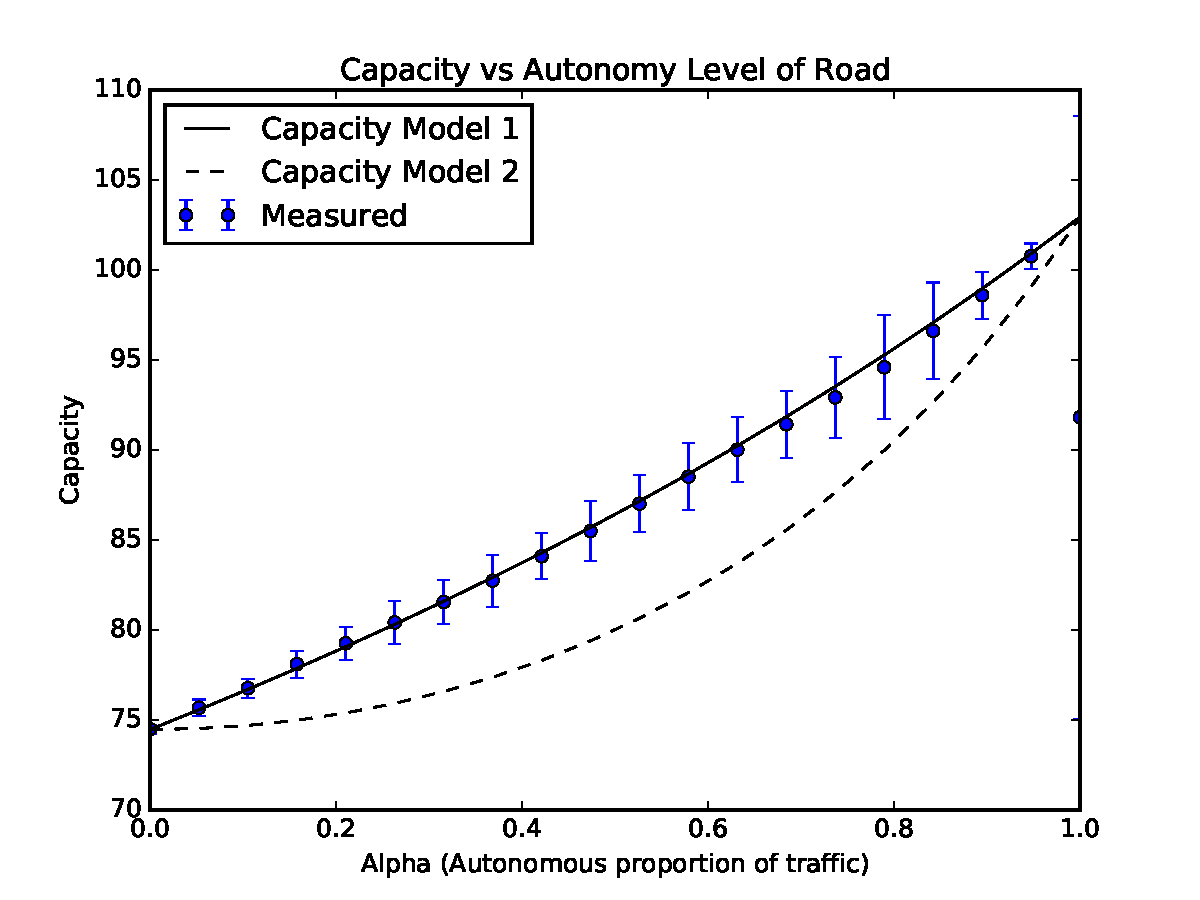
\includegraphics[width = 140mm]{capacity_model1.pdf}
\caption{Road capacity as a function of autonomy level with parameterization of capacity model 1. In this model, autonomous vehicles are indiscriminate in reducing their headway. There is a very strong agreement between the model and the measurements for all values of $\alpha \neq 1$.}
\label{capacity_1}
\end{subfigure}

\begin{subfigure}
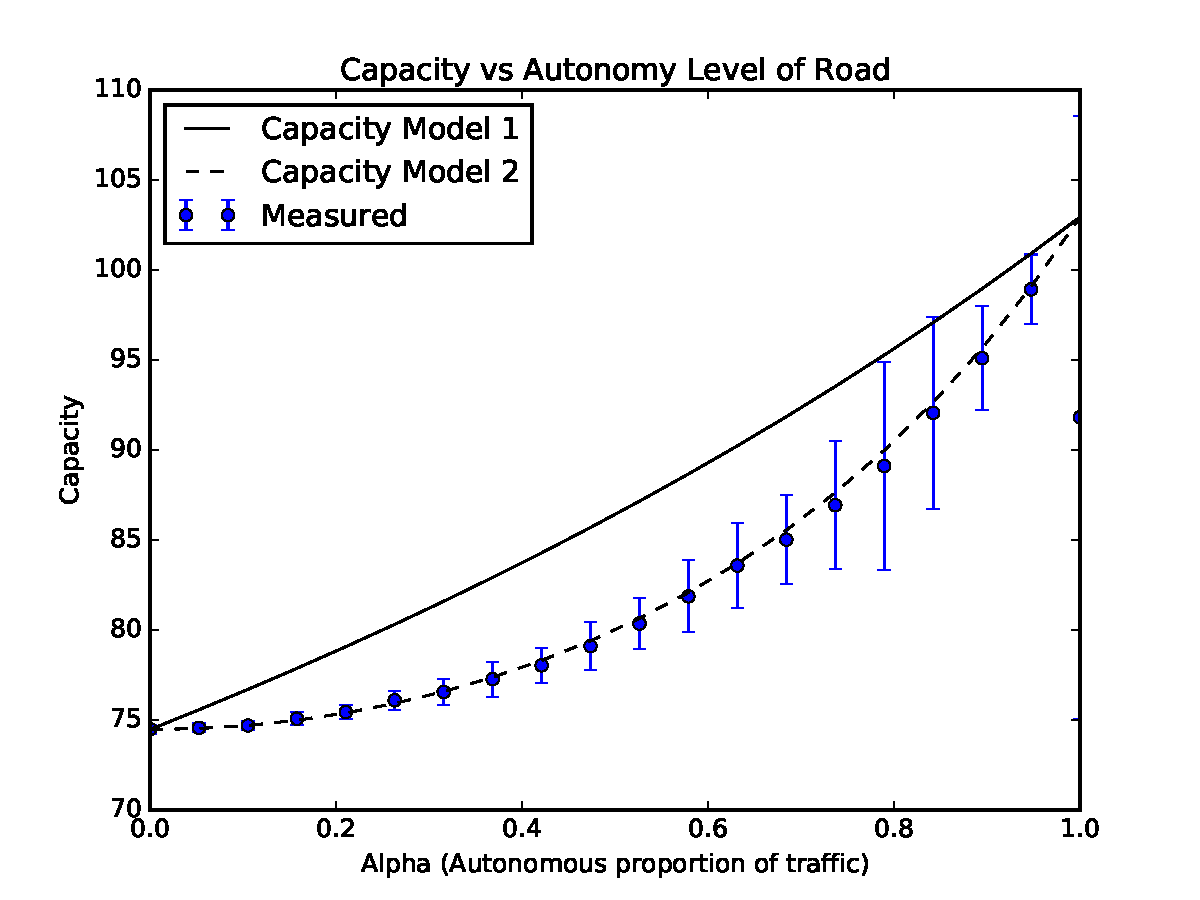
\includegraphics[width = 140mm]{capacity_model2.pdf}
\caption{Road capacity as a function of autonomy level with parameterization of capacity model 2. In this model, autonomous vehicles only reduce their headway if the leading car is also autonomous. There is a very strong agreement between the model and the measurements for all values of $\alpha \neq 1$.}
\label{capacity_2}
\end{subfigure}
\end{figure}

\begin{thebibliography}{10}
\section*{References}
\bibitem{Lazar1}
D. Lazar, S. Coogan, R. Pedarsani, "Capacity Modeling and Routing for Traffic Networks with Mixed Autonomy,"
\newblock \textit{IEEE Conference on Decision and Control (CDC)}, 2017.

\bibitem{SUMO}
D. Krajzewicz, J. Erdmann, M. Behrisch, L. Bieker. "Recent Development and Applications of SUMO - Simulation of Urban MObility,"
\newblock \textit{International Journal On Advances in Systems and Measurements}, 5 (3&4):128-138, 2012.

\bibitem{Varaiya} A. Askari, D. Farias, A. Kurzhanskiy, P. Varaiya, “Effect of Adaptive and Cooperative Adaptive Cruise Control on Throughput of Signalized Arterials,” 
\newblock \textit{arXiv:1703.01657v1}, 2017.

\end{thebibliography}

\appendix
\section{Building Sumo with /ucbtrans/sumo-project}

\subsection{Warnings}
I have only built SUMO with the additions in Ubuntu 16.04, so be warned this may not work on all other systems. Also be warned, it may be possible to get around using some of the mentioned dependencies by disabling certain features of SUMO, or it may be possible to use different packages to suffice for the dependencies, but this worked for me.

\subsection{Setting up the directories}
First, you need to download the \href{https://github.com/ucbtrans/sumo-project}{repository source files} and \href{https://sourceforge.net/projects/sumo/files/sumo/version%200.30.0/}{SUMO 0.30.0}. 
After extracting the files from the Github repository, you can find a directory \verb|sumo-project-master/sumo-0.30.0|, in which you should copy the source files for SUMO 0.30.0. You can simply drag the SUMO 0.30.0 source folder into the sumo-project-master directory, and a reasonable GUI will ask you if you'd like to merge the folders. Make sure \textbf{not} to replace the sumo-project-master files, as these add the IIDM functionality we desire.

\subsection{Dependencies}
Now we are almost ready to compile the project. There are only two dependencies (that I did not already have on a relatively clean system) required to do this. The first is Xerces-C++ (some kind of XML parser). You can install it with the package manager. 
\begin{lstlisting}
sudo apt-get install libxerces-c-dev
\end{lstlisting}
 The second dependency is FOX (some kind of GUI toolkit), which can also be installed via the package manager.
\begin{lstlisting}
sudo apt-get install libfox-1.6-dev
\end{lstlisting}

\subsection{Compiling the project}
To compile the project, you first need to cd into the \verb|sumo-project-master/sumo-0.30.0| directory.
\begin{lstlisting}
cd ~/<specific to you>/sumo-project-master/sumo-0.30.0
\end{lstlisting}
Then, you need to run the \verb|./configure| command.
\begin{lstlisting}
./configure
\end{lstlisting}
Finally, we are ready to make the project. There are a few optional arguments to the make command, although I am not quite sure what we need yet, so I have just used the default settings.
\begin{lstlisting}
make
\end{lstlisting}

If this works successfully, pat yourself on the back. Then, before you get too excited, remember to add the environment variable to your \verb|~/.bashrc| file, so that you can communicate to SUMO with Python. To do this, simply open your bash profile. 
\begin{lstlisting}
gedit ~/.bashrc
\end{lstlisting}
and paste this line into the text file
\begin{lstlisting}
export SUMO_HOME=$\$$HOME/<specific to you>/sumo-project-master/sumo-0.30.0
\end{lstlisting}
Also recommended: paste this line, which will allow you to run SUMO from the command line
\begin{lstlisting}
export PATH=$\$$PATH:$\$$HOME/<specific to you>/sumo-project-master/sumo-0.30.0/bin
\end{lstlisting}

\subsection{Running Examples}
There are Python scripts that run each example, each with a name that starts with "runner." These files can be executed directly if you change the file access permissions to add executability.
\begin{lstlisting}
chmod +x runner.py
\end{lstlisting}
Then you can simply run the example. 
\begin{lstlisting}
./runner.py
\end{lstlisting}
Some of these examples will work right off the bat - like \verb|/example/redLight_simulations|. Some will not. 

\subsubsection{Platoon Bug Fix}
One of the cases I have been able to debug is those examples that use platooning functions. If you run the script without modifying the runner file, you may run into an error complaining that the TraCI module doesn't exist. 

The bug fix is simple - in the \verb|runner.py| file, near the beginning, you will find a line. 
\begin{lstlisting}
from platoon_functions import *
\end{lstlisting}
In the platoon\textunderscore functions file, TraCI is imported, although Python does not yet know where the TraCI module can be found. In the original runner file, after the line shown above, you will see a big try/except statement resembling
\begin{lstlisting}[language=Python]
# import python modules from $\$$SUMO_HOME/tools directory
try:
    ...
except ImportError:
    ...
\end{lstlisting}
This block tells Python where to find your SUMO files. Move the line
\begin{lstlisting}
from platoon_functions import *
\end{lstlisting}
to be below that try/except statement. This should resolve the error and allow TraCI to be imported in the platoon\textunderscore functions module. 

\end{document}
